\section{About Notational Conventions and Schema for \LaTeX~ files}
\label{chap-About-Conventions}

\newthought{When collaborating} with multiple authors using \LaTeX,
conventions about notation and file structures
will save a lot of time.
The schema in Figure~\ref{fg-latex-conventions} already illustrates
a number of conventions that are being  used in this document. 
The list below includes not only the items which are in plain sight in Figure~\ref{fg-latex-conventions}, it also includes items we can observe in subdirectories {\em Algorithms, Figures}, and {\em Tables} as well as the *.tex files in these subdirectories.
\begin{marginfigure}[13ex]%
  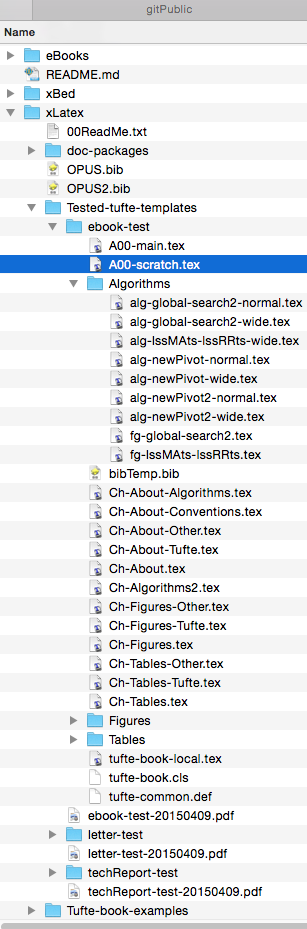
\includegraphics[width=\linewidth]{fg-latex-conventions}
  \caption[Example file fg-latex-conventions.tex]
  {Notational conventions and schema for \LaTeX~files to support collaboration.}
  \label{fg-latex-conventions}
\end{marginfigure}.
%\clearpage
%\small{
\begin{itemize}
\item
Consistently avoid file names with {\em underscore} (\verb+_+).
\item
For complex algorithms, figures and tables, create a separate file which is
prefixed with either \verb+alg-+, \verb+fg-+ or \verb+tb-+
and move the file into the designated subdirectory.
Use the rootname of the file for the label that is used to reference the 
algorithm, figure, or table. For example, we can thus refer to 
contents of file alg-global-search2-normal.tex as 
\verb+Algorithm~\ref{alg-global-search2-normal}+.
Notably, we embed contents of algorithm not only under
\verb+\algorithm+, \verb+\algorithm-wide+ environments but also under 
\verb+\figure+, \verb+\figure*+ environments.
\item
There is always the easy-to-find-file \verb+A00-main.tex+.
This file not only invokes \verb+\documentclass{tufte-book}+
and  the supporting files *tufte*, but also all 
items that are generic to the layout of the book and
new command defitions that are  content-specific with respect to the book.
Finaly, this file also
invokes the book chapters in a well-defined sequence such as 
Ch-About.tex, Ch-Figures.tex, Ch-Tables.tex, and Ch-Algorithms2.tex.
The amount of text in a typical chapter will rarely extend beyond a single page 
since each chapter is likely to invoke
a number of sections that reside in adjacent files and
may represent contributions from several collaborating authors. 
For example, Ch-About.tex invokes four files in this order:
 Ch-About-Conventions.tex,  Ch-About-Tufte.tex, 
  Ch-About-Other.tex,  Ch-About-Algorithms.tex.
\item
The only  *.bib file in the directory ebook-test, bibTemp.bib,
is initially an empty file. 
Within the file \verb+A00-main.tex+, we use relative paths to define
location of the `nearby files' OPUS.bib and OPUS2.bib under xLatex:~
\verb+\bibliography{\detokenize{../../OPUS},+\\
\verb+\detokenize{../../OPUS2}, \detokenize{./bibTemp}}+.\\
Both files, OPUS.bib and OPUS2.bib, are almost always up-to-date
for use by all project participants, so the need for
temporary bib items under the file bibTemp.bib seldom arises.

\end{itemize}
%}